\documentclass[10pt,twocolumn,oneside,a4paper]{article}
\setlength{\columnsep}{10pt}                    %兩欄模式的間距
\setlength{\columnseprule}{0pt}                 %兩欄模式間格線粗細

\usepackage{amsthm}								%定義,例題
\usepackage{amssymb}
\usepackage{fontspec}							%設定字體
\usepackage{color}
\usepackage[x11names]{xcolor}
\usepackage{listings}							%顯示code用的
\usepackage{fancyhdr}							%設定頁首頁尾
\usepackage{graphicx}							%Graphic
\usepackage{enumerate}
\usepackage{titlesec}
\usepackage{amsmath}
\usepackage[CheckSingle, CJKmath]{xeCJK}
 \usepackage{CJKulem}
\usepackage{tikz} % Used for draw Finite Automata

\usepackage{amsmath, courier, listings, fancyhdr, graphicx}
\topmargin=0pt
\headsep=2pt
\textheight=790pt
\footskip=0pt
\voffset=-50pt
\textwidth=545pt
\marginparsep=0pt
\marginparwidth=0pt
\marginparpush=0pt
\oddsidemargin=0pt
\evensidemargin=0pt
\hoffset=-42pt

%\renewcommand\listfigurename{圖目錄}
%\renewcommand\listtablename{表目錄}

%%%%%%%%%%%%%%%%%%%%%%%%%%%%%

\setmainfont{Consolas}
\setmonofont{Consolas}
\setCJKmainfont{Noto Sans CJK TC}
\XeTeXlinebreaklocale "zh"						%中文自動換行
\XeTeXlinebreakskip = 0pt plus 1pt				%設定段落之間的距離
\setcounter{secnumdepth}{3}						%目錄顯示第三層

%%%%%%%%%%%%%%%%%%%%%%%%%%%%%
\makeatletter
\lst@CCPutMacro\lst@ProcessOther {"2D}{\lst@ttfamily{-{}}{-{}}}
\@empty\z@\@empty
\makeatother
\lstset{										% Code顯示
    language=C++,									% the language of the code
    basicstyle=\footnotesize\ttfamily, 					% the size of the fonts that are used for the code
    %numbers=left,									% where to put the line-numbers
    numberstyle=\footnotesize,					% the size of the fonts that are used for the line-numbers
    stepnumber=1,									% the step between two line-numbers. If it's 1, each line  will be numbered
    numbersep=5pt,									% how far the line-numbers are from the code
    backgroundcolor=\color{white},				% choose the background color. You must add \usepackage{color}
    showspaces=false,								% show spaces adding particular underscores
    showstringspaces=false,						% underline spaces within strings
    showtabs=false,								% show tabs within strings adding particular underscores
    frame=false,										% adds a frame around the code
    tabsize=2,										% sets default tabsize to 2 spaces
    captionpos=b,									% sets the caption-position to bottom
    breaklines=true,								% sets automatic line breaking
    breakatwhitespace=false,						% sets if automatic breaks should only happen at whitespace
    escapeinside={\%*}{*)},						% if you want to add a comment within your code
    morekeywords={*},								% if you want to add more keywords to the set
    keywordstyle=\bfseries\color{Blue1},
    commentstyle=\itshape\color{Red4},
    stringstyle=\itshape\color{Green4},
}

%----------------------------------------------------------------------------------------
%   設定 section 行距
%----------------------------------------------------------------------------------------

\makeatletter
\let\origsection\section
\renewcommand\section{\@ifstar{\starsection}{\nostarsection}}

\newcommand\nostarsection[1]
{\sectionprelude\origsection{#1}\sectionpostlude}

\newcommand\starsection[1]
{\sectionprelude\origsection*{#1}\sectionpostlude}

\newcommand\sectionprelude{%
  \vspace{-10pt} % 改這個數字
}
\newcommand\sectionpostlude{%
  \vspace{-10pt} % 改這個數字
}
\makeatother

% ---------------------------------------------------------------------------------------
\usepackage{tocloft}
\cftsetindents{subsection}{1.5em}{2.5em}

\usepackage{fancyhdr}
\pagestyle{fancy}
\fancypagestyle{plain}{
    \fancyhf{}
    \fancyhead[C]{Mashu}
    \fancyhead[L]{National Taiwan Ocean University}
    \fancyhead[R]{(\today) \thepage}
    \renewcommand{\headrulewidth}{0.4pt}
}

\renewcommand{\headrulewidth}{0.4pt}
\renewcommand{\footrulewidth}{0pt}


\begin{document}
\pagestyle{fancy}
\fancyfoot{}
\fancyhead[C]{Mashu}
\fancyhead[L]{National Taiwan Ocean University}
\fancyhead[R]{(\today) \thepage}
\renewcommand{\headrulewidth}{0.4pt}
\renewcommand{\contentsname}{Contents}

\scriptsize
\tableofcontents
\newpage
%%%%%%%%%%%%%%%%%%%%%%%%%%%%%%%%%%%%%%%%%%%%%%%%%%%%%%%%%%%%%%%%%%%%%%%%%%%  BASIC  %%%%%%%%%%%%%%%%%%%%%%%%%%%%%%%%%%%%%%%%%%%%%%%%%%%%%%%%%%%%%%%%%%%%%%%%%%%

\section{Basic}

\subsection{Default code}
\lstinputlisting{basic/Default.cpp}

\subsection{Misc}
\lstinputlisting{basic/Misc.cpp}

\subsection{Fast read \& write}
\lstinputlisting{basic/FastRW.cpp}

\subsection{Sort cmp}
\lstinputlisting{basic/Cmp.cpp}

\subsection{Discretization}
\lstinputlisting{basic/Discretization.cpp}

\subsection{Custom unordered\_map}
\lstinputlisting{basic/CustomUnordered\_map.cpp}

\subsection{\_\_int128 read}
\lstinputlisting{basic/Int128IO.cpp}

\subsection{字典序a嚴格小於b}
\lstinputlisting{basic/LexicographicallySmaller.cpp}

\subsection{Radom}
\lstinputlisting{basic/Random.cpp}

%%%%%%%%%%%%%%%%%%%%%%%%%%%%%%%%%%%%%%%%%%%%%%%%%%%%%%%%%%%%%%%%%%%%%%%%%%%  Matching  %%%%%%%%%%%%%%%%%%%%%%%%%%%%%%%%%%%%%%%%%%%%%%%%%%%%%%%%%%%%%%%%%%%%%%%%%%%
\section{對拍}

\subsection{run.bat}
\lstinputlisting{matching/run.bat}

\subsection{run.sh}
\lstinputlisting{matching/run.sh}
%%%%%%%%%%%%%%%%%%%%%%%%%%%%%%%%%%%%%%%%%%%%%%%%%%%%%%%%%%%%%%%%%%%%%%%%%%%  Flow  %%%%%%%%%%%%%%%%%%%%%%%%%%%%%%%%%%%%%%%%%%%%%%%%%%%%%%%%%%%%%%%%%%%%%%%%%%%
\section{Flow \& Matching}

\subsection{Dicnic}
\lstinputlisting{flow/Dicnic.cpp}

\subsection{ZKW FLow}
\lstinputlisting{flow/ZkwFlow.cpp}

\subsection{Hungarian}
\lstinputlisting{flow/Hungarian.cpp}

\subsection{KM}
\lstinputlisting{flow/KM.cpp}

%%%%%%%%%%%%%%%%%%%%%%%%%%%%%%%%%%%%%%%%%%%%%%%%%%%%%%%%%%%%%%%%%%%%%%%%%%%  Graph  %%%%%%%%%%%%%%%%%%%%%%%%%%%%%%%%%%%%%%%%%%%%%%%%%%%%%%%%%%%%%%%%%%%%%%%%%%%
\section{Graph}

\subsection{BCC}
\lstinputlisting{graph/BccVertex.cpp}

\subsection{SCC}
\lstinputlisting{graph/SCC.cpp}

\subsection{2SAT}
\lstinputlisting{graph/2SAT.txt}

\subsection{MaximalClique}
\lstinputlisting{graph/MaximalClique.cpp}

\subsection{MaximumClique}
\lstinputlisting{graph/MaximumClique.cpp}

\subsection{Minimum Mean Cycle}
\lstinputlisting{graph/Minimum Mean Cycle.cpp}

\subsection{Dominator Tree}
\lstinputlisting{graph/Dominator Tree.cpp}
%%%%%%%%%%%%%%%%%%%%%%%%%%%%%%%%%%%%%%%%%%%%%%%%%%%%%%%%%%%%%%%%%%%%%%%%%%%  DP  %%%%%%%%%%%%%%%%%%%%%%%%%%%%%%%%%%%%%%%%%%%%%%%%%%%%%%%%%%%%%%%%%%%%%%%%%%%
\section{DP}

\subsection{數位DP}
\lstinputlisting{DP/digitDP.cpp}

%%%%%%%%%%%%%%%%%%%%%%%%%%%%%%%%%%%%%%%%%%%%%%%%%%%%%%%%%%%%%%%%%%%%%%%%%%%  Math  %%%%%%%%%%%%%%%%%%%%%%%%%%%%%%%%%%%%%%%%%%%%%%%%%%%%%%%%%%%%%%%%%%%%%%%%%%%
\section{Math}

\subsection{Formulas}
\lstinputlisting{math/Formula.txt}

\subsection{Primes}
\lstinputlisting{math/Primes.txt}

\subsection{Quick Pow}
\lstinputlisting{math/QuickPow.cpp}

\subsection{Mat quick Pow}
\lstinputlisting{math/MatPow.cpp}

\subsection{Primes Table}
\lstinputlisting{math/PrimesTable.cpp}

\subsection{Factor Table}
\lstinputlisting{math/FactorTable.cpp}

\subsection{Catalan Number}
\lstinputlisting{math/CatalanNumber.cpp}

\subsection{Miller Rabin}
\lstinputlisting{math/MillerRabin.cpp}

\subsection{PollarRho}
\lstinputlisting{math/PollardRho.cpp}

\subsection{PrimeFactorO(logn)}
\lstinputlisting{math/PrimeFactorO(logn).cpp}

\subsection{O(1)mul}
\lstinputlisting{math/O(1)mul.cpp}

\subsection{Josephus Problem}
\lstinputlisting{math/JosephusProblem.cpp}

\subsection{Harmonic Sum}
\lstinputlisting{math/HarmonicSum.cpp}

%%%%%%%%%%%%%%%%%%%%%%%%%%%%%%%%%%%%%%%%%%%%%%%%%%%%%%%%%%%%%%%%%%%%%%%%%%%  DataStructure  %%%%%%%%%%%%%%%%%%%%%%%%%%%%%%%%%%%%%%%%%%%%%%%%%%%%%%%%%%%%%%%%%%%%%%%%%%%
\section{Data Structure}

\subsection{BIT}
\lstinputlisting{dataStructure/BIT.cpp}

\subsection{Sparse Table}
\lstinputlisting{dataStructure/Sparse Table.cpp}

\subsection{Segment Tree}
\lstinputlisting{dataStructure/SegmentTree.cpp}

\subsection{持久化線段樹}
\lstinputlisting{dataStructure/persistent_seg_tree.cpp}

\subsection{Time Segment Tree}
\lstinputlisting{dataStructure/TimeSegmentTree.cpp}

\subsection{Treap}
\lstinputlisting{dataStructure/Treap.cpp}

\subsection{PBDS}
\lstinputlisting{dataStructure/PBDS.cpp}

%%%%%%%%%%%%%%%%%%%%%%%%%%%%%%%%%%%%%%%%%%%%%%%%%%%%%%%%%%%%%%%%%%%%%%%%%%%  String  %%%%%%%%%%%%%%%%%%%%%%%%%%%%%%%%%%%%%%%%%%%%%%%%%%%%%%%%%%%%%%%%%%%%%%%%%%%
\section{String}

\subsection{SA}
\lstinputlisting{string/SA.cpp}

\subsection{KMP}
\lstinputlisting{string/KMP.cpp}

\subsection{Single Hash}
\lstinputlisting{string/SingleHash.cpp}

\subsection{Double Hash}
\lstinputlisting{string/DoubleHash.cpp}

\subsection{Trie}
\lstinputlisting{string/Trie.cpp}

\subsection{Z value}
\lstinputlisting{string/Zvalue.cpp}

\subsection{MinRotation}
\lstinputlisting{string/MinRotation.cpp}

\subsection{Manacher}
\lstinputlisting{string/Manacher.cpp}

\subsection{PalTree}
\lstinputlisting{string/PalTree.cpp}

\subsection{DistinctSubsequence}
\lstinputlisting{string/DistinctSubsequence.cpp}
%%%%%%%%%%%%%%%%%%%%%%%%%%%%%%%%%%%%%%%%%%%%%%%%%%%%%%%%%%%%%%%%%%%%%%%%%%%  Tree  %%%%%%%%%%%%%%%%%%%%%%%%%%%%%%%%%%%%%%%%%%%%%%%%%%%%%%%%%%%%%%%%%%%%%%%%%%%
\section{Tree}

\subsection{TreeHash}
\lstinputlisting{tree/TreeHash.cpp}

\subsection{輕重鏈剖分}
\lstinputlisting{tree/heavyLightDecomposition.cpp}
%%%%%%%%%%%%%%%%%%%%%%%%%%%%%%%%%%%%%%%%%%%%%%%%%%%%%%%%%%%%%%%%%%%%%%%%%%%  Geometry  %%%%%%%%%%%%%%%%%%%%%%%%%%%%%%%%%%%%%%%%%%%%%%%%%%%%%%%%%%%%%%%%%%%%%%%%%%%
\section{Geometry}

\subsection{Definition2D}
\lstinputlisting{geometry/Definition2D.cpp}

\subsection{Basic}
\lstinputlisting{geometry/Basic.cpp}

\subsection{PolygonArea}
\lstinputlisting{geometry/PolygonArea.cpp}

\subsection{IsPointInPolygon}
\lstinputlisting{geometry/IsPointInPolygon.cpp}

\subsection{ConvexHull}
\lstinputlisting{geometry/ConvexHull.cpp}

\subsection{ConvexHullTrick}
\lstinputlisting{geometry/ConvexHullTrick.cpp}

\subsection{Polar Sort}
\lstinputlisting{geometry/PolarSort.cpp}

\subsection{PickTheorm}
\lstinputlisting{geometry/PickTheorm.cpp}

\subsection{最近點對}
\lstinputlisting{geometry/ClosestEuclideanDistance.cpp}

\subsection{幾何中位數}
\lstinputlisting{geometry/Weiszfeld.cpp}

\subsection{矩陣掃描線}
\lstinputlisting{geometry/SweepLine.cpp}

\subsection{Circle Definition}
\lstinputlisting{geometry/CircleDefinition.cpp}

\subsection{CircleCover}
\lstinputlisting{geometry/CircleCover.cpp}
%%%%%%%%%%%%%%%%%%%%%%%%%%%%%%%%%%%%%%%%%%%%%%%%%%%%%%%%%%%%%%%%%%%%%%%%%%%  SpecialQuestion  %%%%%%%%%%%%%%%%%%%%%%%%%%%%%%%%%%%%%%%%%%%%%%%%%%%%%%%%%%%%%%%%%%%%%%%%%%%
\section{特殊題目}

\subsection{包含子字串計數}
\lstinputlisting{SpecialQuestion/ContainString.cpp}
%%%%%%%%%%%%%%%%%%%%%%%%%%%%%%%%%%%%%%%%%%%%%%%%%%%%%%%%%%%%%%%%%%%%%%%%%%%  Python  %%%%%%%%%%%%%%%%%%%%%%%%%%%%%%%%%%%%%%%%%%%%%%%%%%%%%%%%%%%%%%%%%%%%%%%%%%%
\section{Python}

\subsection{Decimal}
\lstinputlisting{python/Decimal.py}

\subsection{Fraction}
\lstinputlisting{python/Fraction.py}

\subsection{Misc}
\lstinputlisting{python/Misc.py}
\onecolumn
\centering
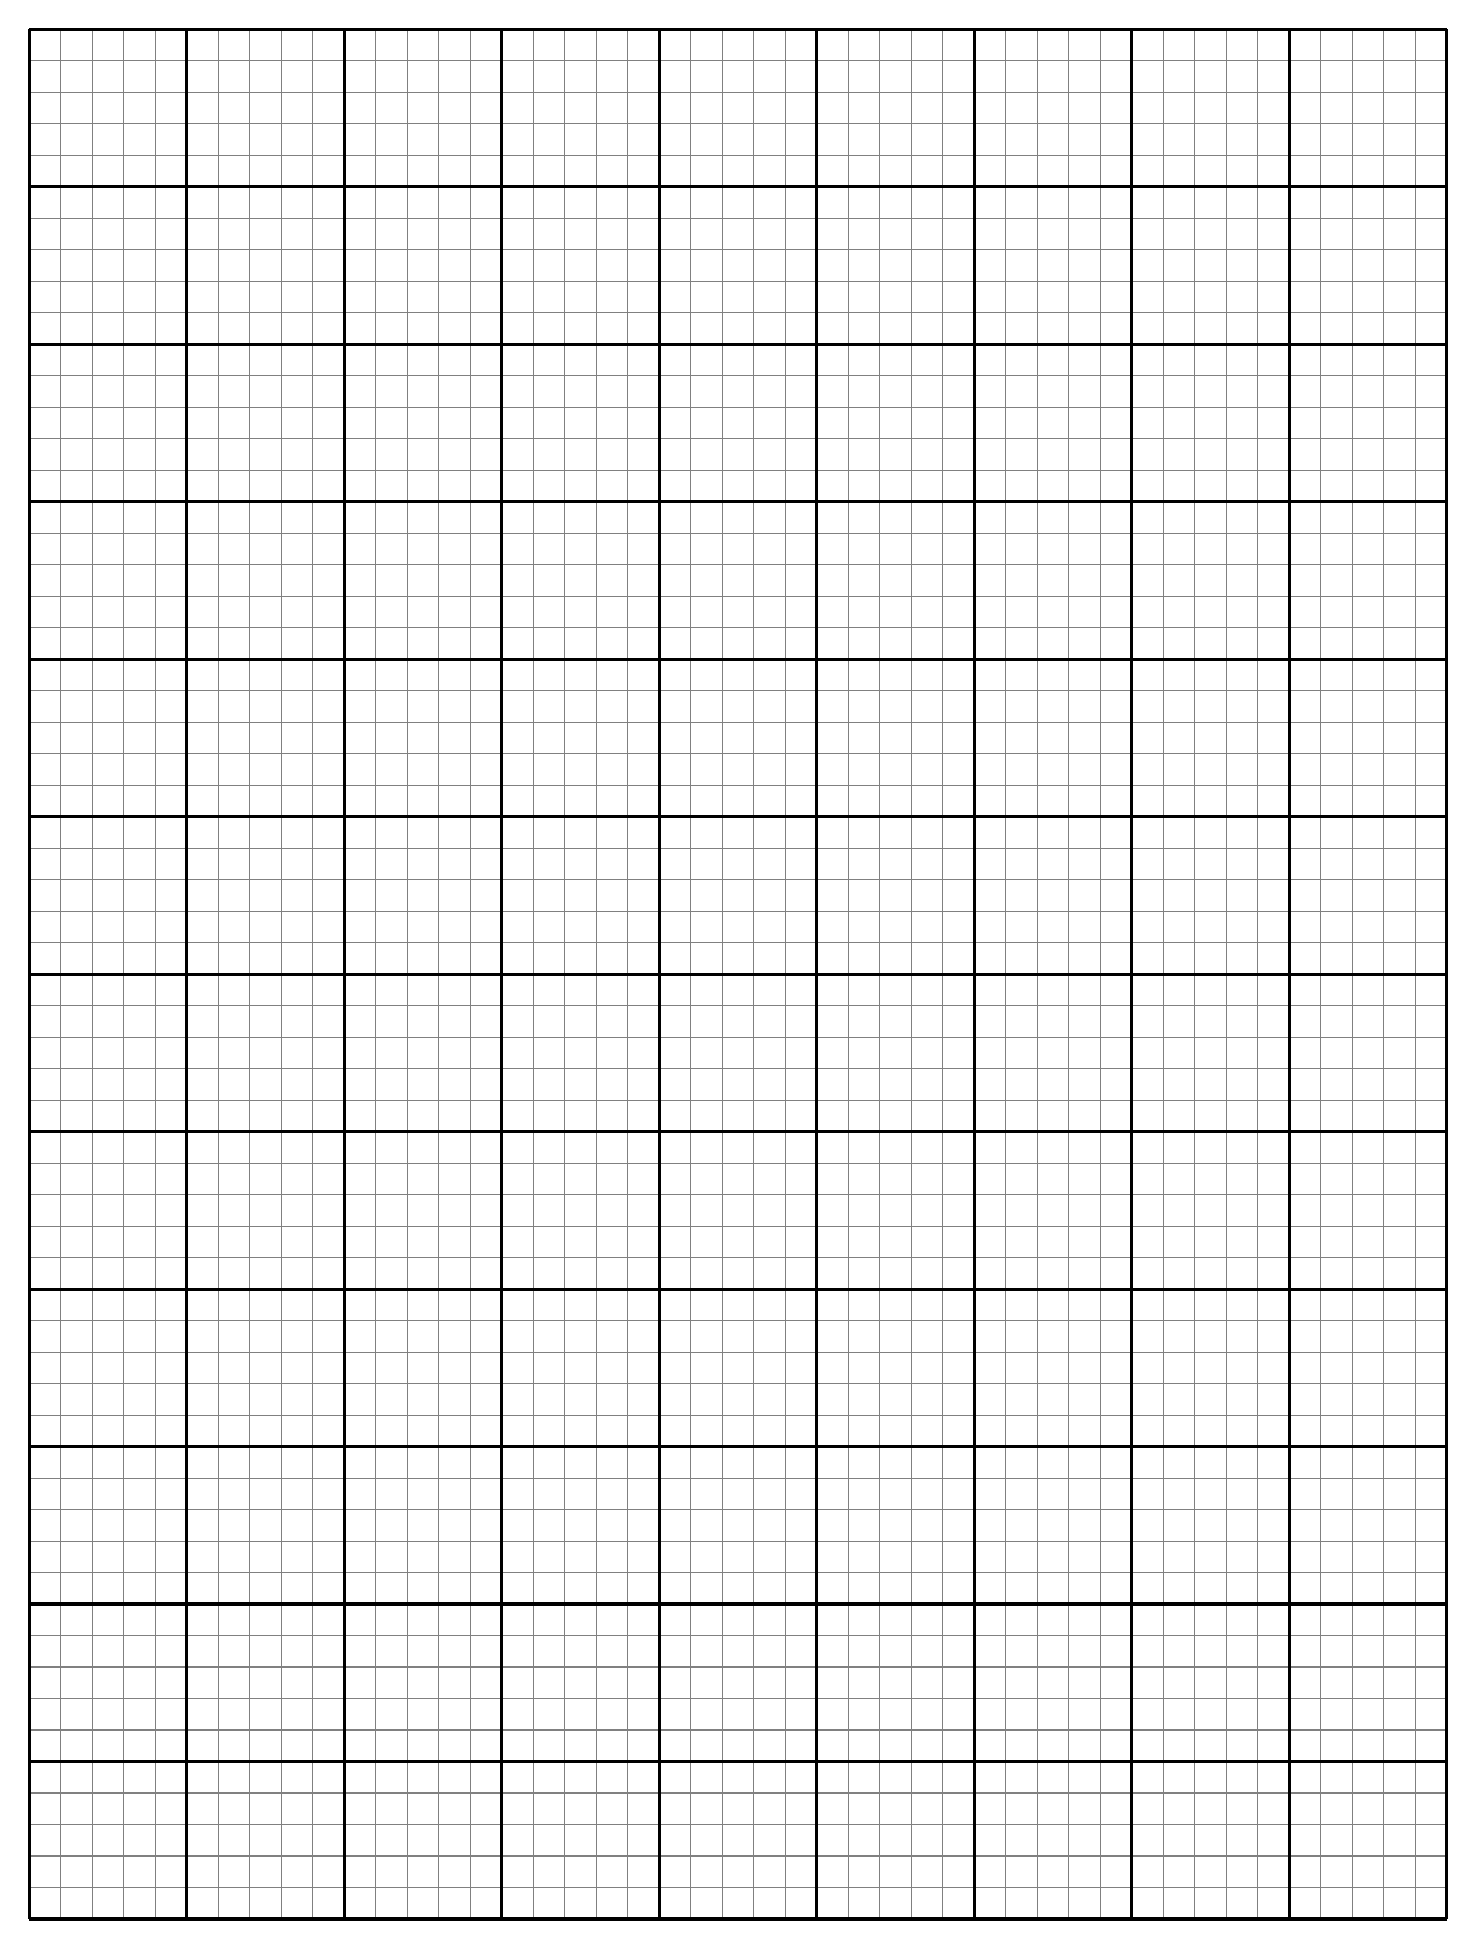
\begin{tikzpicture}[every node/.style={minimum size=1cm-\pgflinewidth, outer sep=10pt}, scale=2]
    \draw[step=0.2cm,color=gray] (0,0) grid (9,12);
    \draw[step=1cm,color=black,line width=0.4mm] (0,0) grid (9,12);
\end{tikzpicture}

\centering
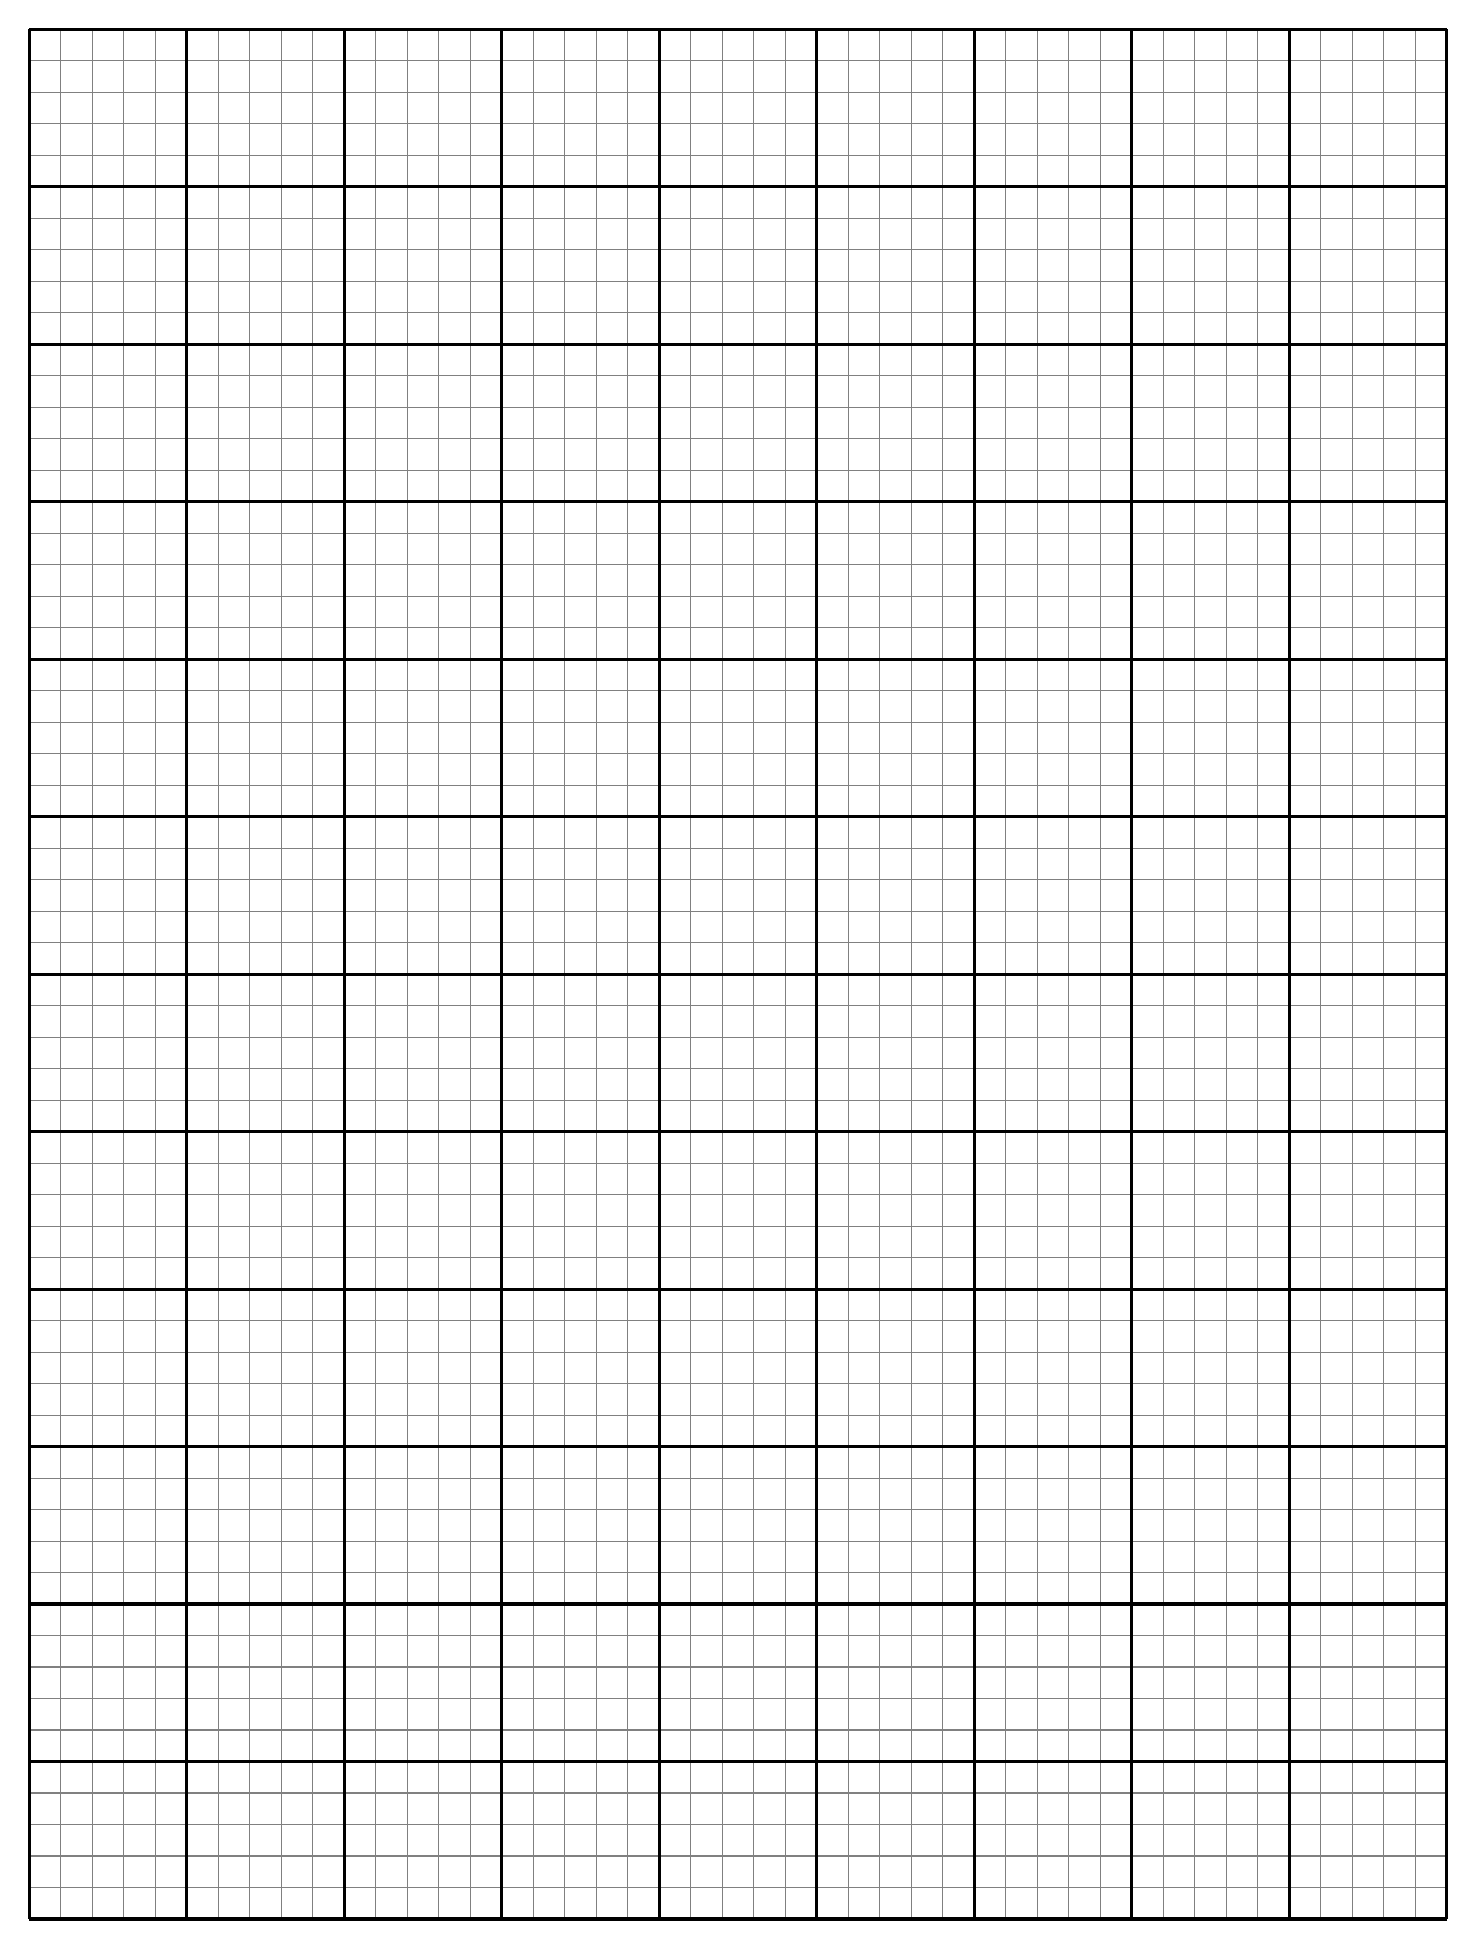
\begin{tikzpicture}[every node/.style={minimum size=1cm-\pgflinewidth, outer sep=10pt}, scale=2]
    \draw[step=0.2cm,color=gray] (0,0) grid (9,12);
    \draw[step=1cm,color=black,line width=0.4mm] (0,0) grid (9,12);
\end{tikzpicture}


\end{document}
